\documentclass[fleqn,a4paper,8pt,papersize]{jsarticlek}
\usepackage{amsmath,amssymb,multicol}
\usepackage{zogeny,ceo}
\setlength\fullwidth{52zw}
\setlength\textwidth{\fullwidth}
\setlength{\textheight}{45\baselineskip}

\begin{document}
\ceorb{ymawarikomi}\textgt{の紹介}\\
ymawarikomiの基本のプログラムは\\
\begin{Verbatim}
\def\ymawarikomi#1#2#3#4#5#6{%
  \par %
  \begingroup\clubpenalty=150
  \def\par{\endgraf\endgroup}%
  \noindent\hangindent-#1zw\hangafter=-#2%
		\raisebox{-#5}[0pt][0pt]{%
          \hbox to 0pt{\hskip#6zw\includegraphics[width=#3]{#4}\hss}}}
\end{Verbatim}
です．下の記号\yy clipを作るときに米村昭芳氏（駿台講師）に教わった方法を変形しました．元はクヌースのThe TeXbookにあるプログラムです．このように短いコマンドで回り込みができるというのはすごいと思いませんか？TeXを始めたとき，図や表の回り込みが容易にはできないことに驚きました．これならWordの方がはるかにましだと．．．回り込みのスタイルはいくつか知られています．
wrapfig，emathのスタイルなどがありますが．．．

ceosty内であれば，字下げをしている環境（リスト系環境など）でも使えるようにしました．普通のリスト系環境は字下げをparshapeで行っていますが，それをleftskip，rightskipで行ったのです．

\begin{multicols}{2}
\begin{waku}
\ymawarikomi{12}{7}{3.5cm}{fig2-1.eps}{3.5cm}{12}%
以前のwaku環境ではこの回り込みは有効ではありませんでした．解決のためにwaku環境を手直ししました．字下げをしていたindentスタイルを別のものに変えたのです．現在はオリジナルのindentスタイルではありません．回り込みコマンドの後に本文を続ける場合はパーセントマークを入れてください．奇妙な空きが入るのを防ぎます．
\clip このclipは旺文社の入試正解のコメント欄で使われているものを真似しました．ただし，入試正解がどんなコマンドになっているのかは私たちも教えてもらってはいません．clip,ymawarikomiはceostyの枠で囲むときは，どの枠も使えます．
\end{waku}

\kakkoichib \quad 使い方
ymawarikomiの引数は6つです．右に何文字分空けるか，回り込みの行数，読み込み図の左右のサイズ，図の名前，その図を何センチ下に下げるか，図を右にどれだけ移動するかです．受験雑誌「大学への数学」の場合ですと，図の基本サイズは7行12字，左から13字空けて，7行取り，図は4.5センチの透明の正方形内に描き，印刷仕上がりは3.5センチですから，13,7,3.5cm,図の名前,3.5cm,13と入れます．図はそのコマンドを入れたところに右寄せで入ります．
\verb/\ymawarikomi{12}{7}{3.5cm}/

\verb/{fig2-1.eps}{3.5cm}{13}/

となります．
\ymawarikomi{12}{7}{3.5cm}{fig2-1.eps}{3.5cm}{13.5}%
ああああああああああああああああああああああああああああああああああああああああああああああああああああああああああああああああああああああああああああああああああああああああああああああああああああああああああああああああああ\\
\kakkonib \quad リスト系環境でも使える

通常，こうした回り込みは段落を成形してある環境（リスト系環境）ではemathの大熊氏作のmawarikomiスタイルを除いて，字下げが効きません．しかし，ymawarikomiはceosty内であれば使えます．

\begin{mondai}リスト系環境ではこのように字下げが行われます．
\begin{shomon}
正しく字下げが行われる．正しく字下げが行われる．
\end{shomon}
\begin{shomon}
\ymawarikomi{10}{6}{3.5cm}{fig2-1.eps}{3cm}{12}%
正しく字下げが行われる．正しく字下げが行われる．
正しく字下げが行われる．正しく字下げが行われる．
正しく字下げが行われる．正しく字下げが行われる．
正しく字下げが行われる．正しく字下げが行われる．
\end{shomon}
\end{mondai}
\aki(40,0)

\kakkosanb \quad 図や表を左右に並べる

\RESETKEYA
\setkeys{zogen}{%
hensu=表さ,kansub=あ,kansuc=い,kansud=う,
ranaa=a,ranab=b,ranac=c,
ranbb=a,ranbc=0}
ymawarikomiは図や表を2つ横に並べるときも簡単です．図を左右のずれと上下のずれ（一行分）を考えて入れ,
図の上下幅分だけvspaceで空けるだけです．ただし，このとき，ymawarikomiなどのコマンドを入れたら，空行を作って次の本文との間を空けてください．
\ymawarikomi{14}{7}{3.5cm}{fig2-1.eps}{3.5cm}{14}
\hmawarikomi{0}{7}{\hspace{-4zw}
\zogen(4,3)}{1cm}{0}
\vspace{6\baselineskip}

\begin{Verbatim}
\ymawarikomi{14}{7}{3.5cm}{fig2-1.eps}{3.5cm}{14}
\hmawarikomi{0}{7}{\hspace{-4zw}
\zogen(4,3)}{1cm}{0}
\vspace{6\baselineskip}
\end{Verbatim}

epsでないもの（たとえば表）を入れるときの回り込みはhmawarikomiです．

\vspace{1\baselineskip}
\begin{Verbatim}
\def\hmawarikomi#1#2#3#4#5{%
\par
  \begingroup\clubpenalty=150
  \def\par{\endgraf\endgroup}%
  \noindent
  \hangindent-#1zw\hangafter=-#2%
  \raisebox{-#4}[0pt][0pt]{%
     \hbox to 0pt{\hskip#5zw{#3}\hss}}}
\end{Verbatim}

hmawarikomiの引数は5つです．左から何文字空けるか，回り込みの行数，入れるもの，それを何センチ下に下げるか，右にどれだけずらすかです．
置換積分の表を入れてみましょう．\\
\verb/\hmawarikomi{10}{3}/\\
\verb/{\hskip3zw\chikan}{0.3cm}{11}/
\RESETKEYD
\hmawarikomi[\hskip12zw 置換の表]{10}{3}{\hskip3zw\chikan}{1cm}{11}%
ああああああああああああああああああああああああああああああああああああああああああああああああああああ\\

\kakkoshib \quad 図にキャプション

図にキャプションをつけることもできます．[\ ]で囲って先頭に入れてください．ただし，大学受験の数学では基本的にキャプションを使わないので積極的に設定してありません．使う人が好みに合わせてカスタマイズしてください．hmawarikomiは上に，ymawarikomiは下につきます．統一したいのですが，現段階では位置あわせがうまくできていません．基本的にhmawarikomiは表などの汎用仕様，ymawarikomiはeps特定仕様にしてあります．表などでは上下サイズを検出することが（しようと思えばできるけど，面倒なので）やってなく，キャプションを下につけるための自動化の手抜きをしているのです．

\kakkogob \quad 改段落後の回り込み

\quad 改段落して回り込みを続けることもできます．
\ymawarikomi[図キャプション]{13}{7}{3.5cm}{fig2-1.eps}{3cm}{13}%
ここからここからここから
ここからここからここからここからここからここからここまで．\\

空行を空けて改段落すると回り込みが切れ，次の小問に移ると下の段落と重なります．この場合に回り込みを継続したいときは次の小問でhmawarikomi(13,2)のように残りの回り込みを打ち込んでください．

なお，単なる改行の場合は\yy \yy を用いると回り込みが継続します．

単なる改段落するけれど，回り込みを続けたいときで，本当に行間を空けたいとき．
\ymawarikomi[図だよ]{13}{8}{3.5cm}{fig2-1.eps}{3.5cm}{13}%
ここからここからここからここからここからここからここまで．\\
\aki(25,5)\quad 改段落したように見える．改段落したように見える．改段落したように見える．改段落したように見える．改段落したように見える．改段落したように見える．この場合の改行には\yy \yy を用いている．行間の空きには幅が0の支柱を立てるaki(25,5)を用いた．

\begin{waku}
\begin{reidai}
waku環境でymawarikomiは使える．
\begin{shomonr}
字下げが無視されない．
\end{shomonr}
\begin{shomonr}
\ymawarikomi{11}{6}{3.5cm}{fig2-1.eps}{2.5cm}{9}%
字下げが正しく行われる．
字下げが正しく行われる．
字下げが正しく行われる．
字下げが正しく行われる．
字下げが正しく行われる．
字下げが正しく行われる．行われる.

\end{shomonr}
\end{reidai}
\end{waku}

なお，waku環境にする前後は空行を入れましょう．
\\
\\
\kakkorokub \quad minipageについて

次はminipageで回り込みらしくする伝統的な方法の説明をします．
次にはminipageで図を入れてみます．左段に幅12字で本文，右段に幅12字で図を入れます．1字分はロスです．\\
minipageを入れると行間が妙に詰まったり，空いたりしますので，aki(x,y)で適当に空けます．ここではminipage始まりは行間の調整をしていないので，詰まっています．minipage終わりは行間の調整をしたので，空きが適当（ちょうどよい）です．\\
\begin{minipage}{12zw}
minipageの左側ああああああああああああああああああああああああああああああああああああああああああああああああああああああああああああああああああああああああああ．
\end{minipage}
\begin{minipage}{12zw}
\ \ 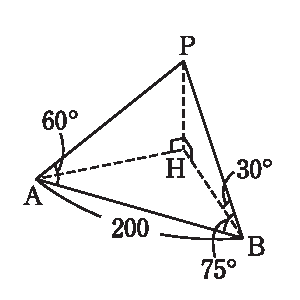
\includegraphics[width=3.5cm]{fig2-1.eps}
\end{minipage}\\
\aki(15,0)%
どの形式でも，多少の試行錯誤は必要です．それぞれに慣れが必要で，きっとどれもこれも一長一短です．それぞれに慣れが必要で，きっとどれもこれも一長一短です．あああああああああああああああああああああああああああああああああああああああああああああああああああああああああああああああああああああああああああああああああああああああああああああああああああああああああああああああああああああああああああああああああああああああああああああああああ．あああああああああああああああああああああああああああああああああああああああああああああああああああああああああああああああああああああああああああああああああああああああああああああああああああああああああああああああああああああああああああああああああああああああああああああああああ．あああああああああああああああああああああああああああああああああああああああああああああああああああああああああああああああああああああああああああああああああああああああああああああああああああああああああああああああああああああああああああああああああああああああああああああああああ．
\end{multicols}
\end{document}